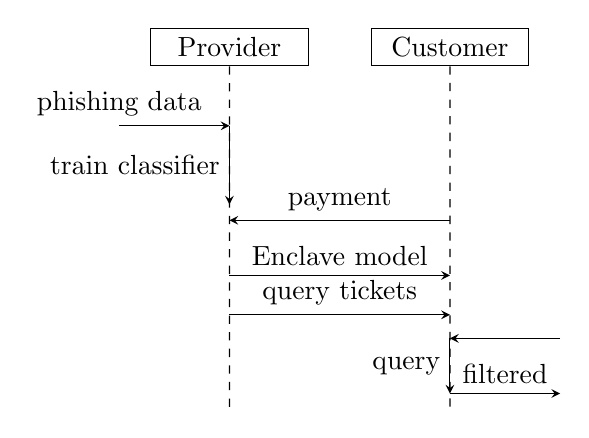
\begin{tikzpicture}[>=stealth, xscale=0.35]
    \draw (-4,0) node[draw, minimum width=2cm] (provider) {Provider};
	\draw[dashed] (provider) -- ++(0,-4.6);

    \draw (4,0) node[draw, minimum width=2cm] (customer) {Customer};
	\draw[dashed] (customer) -- ++(0,-4.6);

	\draw[->] (-8,-1) -- (-4,-1) node[above, pos=0] {phishing data};
	\draw[->] (-4,-1) -- (-4,-2) node[left, midway] {train classifier};

	\draw[->] (4,-2.2) -- (-4,-2.2) node[above, midway] {payment};
	\draw[->] (-4,-2.9) -- (4,-2.9) node[above, midway] {Enclave model};
	\draw[->] (-4,-3.4) -- (4,-3.4) node[above, midway] {query tickets};

	\draw[->] (8,-3.7) -- (4,-3.7) node[above, midway] {\mail{}};
	\draw[->] (4,-3.7) -- (4,-4.4) node[left, midway] {query};
	\draw[->] (4,-4.4) -- (8,-4.4) node[above, midway] {filtered};
\end{tikzpicture}
